\documentclass[11pt]{article}

\usepackage[a4paper,margin=2.6cm]{geometry}
\usepackage[T1]{fontenc}
\usepackage[utf8]{inputenc}
\usepackage{lmodern}
\usepackage{microtype}
\usepackage{amsmath,amssymb}
\usepackage{booktabs}
\usepackage{graphicx}
\usepackage{xcolor}
\usepackage[font=small,labelfont=bf]{caption}
\usepackage{enumitem}
\definecolor{linkblue}{HTML}{1c5cab}
\usepackage[colorlinks=true,linkcolor=linkblue,citecolor=linkblue,urlcolor=linkblue]{hyperref}

\newcommand{\sillage}{\textsc{Sillage}}
\newcommand{\ci}[2]{{\footnotesize[#1,\,#2]}}

\title{\bfseries Stored Is Not Recalled:\\
Behavioral Laws of a Gradient-Free Memory\\
for Frozen Language Models}
\author{Abderrahmane Sghairi\\
\small Independent Researcher, Issoire, France\\
\small \texttt{sghairipro63@gmail.com}}
\date{August 2026 --- v2 (adds the capacity test, \S\ref{sec:capacity})\\[2pt]
\small DOI: \href{https://doi.org/10.5281/zenodo.22125859}{10.5281/zenodo.22125859}
\qquad Code: \href{https://github.com/riscoss63/sillage}{github.com/riscoss63/sillage}}

\begin{document}
\maketitle

\begin{abstract}
Perplexity gains can coexist with a memory that changes no behavior, and recent work has made behavioral evaluation a requirement for test-time-memory claims. This paper is the behavioral anatomy of the \sillage{} system --- the gradient-free, fixed-size memory of five companion papers --- measured with an instrument whose control is built in: invented facts the base models cannot know, probed by free completion with the supporting context absent, on frozen GPT-2 and Qwen3-0.6B. Six laws emerge, each with its mechanism attributed. \textbf{(1) Stored is not recalled: behavioral conversion is a trust problem.} After a correcting document, Qwen3's recall of updated facts plateaus at 20\% over four readings --- yet raising only the readout's interpolation weight on the \emph{same state, with no new reads}, takes it to 100\% and repairs its residual recall failures too. The same mechanism explains, in one stroke, why kNN-LM's likelihood gains never move the argmax, why the semantic tier improves likelihood but not recall, and why calibration governs speculative acceptance. \textbf{(2) The paraphrase boundary is structural, not a trust problem}: 0\% under every setting tested, including maximal readout trust --- the two failure modes are now experimentally separated. \textbf{(3) The Hebbian matrix is working memory; the exact cold store is durable memory}: alone, the matrix's recall erodes from 90\% to 17\% under 110k tokens of interference (to 0\% with forgetting enabled) while the cold tier holds 97\% throughout --- so leaky forgetting is behaviorally free, and consolidation-by-surprise is the retention mechanism, not a bonus. The rank-16 adapter memorizes nothing (0\% everywhere): facts live in the memory, style in the readout. \textbf{(4) The two-occurrence rule}: facts seen once never clear the cold store's admission threshold and die with the working memory (0\% by +43k); seen twice, they are retained at 90--100\% through +110k. A design constant becomes a behavioral law: this system durably remembers what it has seen twice. \textbf{(5) Context equivalence has two regimes}: on documents the state has read, the bare model never matches memory-plus-64-tokens even with $16\times$ the context (perplexity 65 vs 4.8 --- the answer is not in the local window); on an edited sibling never read, the bare model needs $C^{*}\!=195$ tokens to match it, and the memory still helps at full context ($-25\%$). \textbf{(6) The surprise gate is an intrinsic adversarial defense}: bulk collision attacks at the facts' own addresses self-neutralize because in-window repetition becomes predictable to the frozen model and is priced at nearly zero --- nine attack writes bought a third of their nominal mass, and the write-level trace verifies the amplitude rule exactly while locating the vulnerable channel in the cold tier's gate-blind counts, yielding a principled fix (surprise mass per successor). All results are deterministic under fixed seeds, every number is committed as JSON, and the instrument, its predictions registered before each run, is released. \textbf{Version 2 adds the capacity test}: one state written by Qwen3-0.6B, served by 0.6B, 1.7B and 4B under an identical stack --- at published trust, conflict resolution is 10\% at all three sizes; at calibrated trust, 100\% at all three. Capacity does not buy conversion; the readout does, and at 4B the whole trust dial compresses into the abstention threshold alone.
\end{abstract}

\section{Introduction}

The companion papers of this series equipped frozen language models with a gradient-free, fixed-size memory --- a Hebbian matrix with vector-symbolic $n$-gram keys and amplitude values \cite{sillage}, a score-routed semantic tier \cite{router}, a cold store consolidated by surprise mass \cite{hier}, a delta-rule readout adapter \cite{fw}, and, most recently, cross-model transfer and exact speculative acceleration from the same state \cite{drafter}. Their currency was overwhelmingly \emph{likelihood}, plus one recall task. That is no longer sufficient grounds for a memory claim: likelihood improvements can leave behavior untouched --- kNN-LM's gains famously do not move greedy decisions \cite{sillage,khandelwal2020} --- and a recent evaluation framework demonstrates test-time updates that lower perplexity while free recall stays at zero, proposing an evidence ladder of behavioral probes: later recall, paraphrase robustness, retention, locality, conflict handling, and use with the supporting context removed \cite{beyondppl}.

This paper climbs that ladder for the whole \sillage{} system, and finds that the interesting question is not \emph{whether} the memory changes behavior (it does: from 11.3\% to 23.7\% content recall in \cite{sillage}) but \emph{what governs the conversion} of stored information into behavior, tier by tier. The instrument is deliberately simple: thirty invented facts --- entities no base model can know, so the control is built into the design --- embedded in filler, read once by the tool, and probed by greedy completion with the supporting text absent. Every probe is deterministic under fixed seeds; predictions were registered in the experiment log before each run; and two of the results below were reached by refusing to believe a measurement that flattered the system (\S\ref{sec:adversarial}).

\paragraph{Contributions.} Six behavioral laws, each with its mechanism attributed by ablation, decomposition, or write-level instrumentation:
\begin{enumerate}[leftmargin=1.5em,itemsep=2pt]
\item \textbf{Stored is not recalled} (\S\ref{sec:trust}): a conflict-resolution plateau (20\% after four corrective readings on Qwen3) vanishes --- 100\%, zero new reads --- when only the readout's trust is raised; the finding unifies three previously separate observations across the series.
\item \textbf{Two boundaries of different natures} (\S\ref{sec:boundaries}): paraphrase failure is invariant to trust (structural: the keys), while conflict failure is pure trust (the readout) --- separated experimentally for the first time.
\item \textbf{Working memory vs durable memory} (\S\ref{sec:whocarries}): a four-voice decomposition over 110k tokens of interference shows the matrix eroding ($90 \to 17\%$ alone; $0\%$ under forgetting) while the cold store holds 97\% constant --- making leaky forgetting behaviorally free and consolidation the retention mechanism; the adapter stores no facts at all.
\item \textbf{The two-occurrence rule} (\S\ref{sec:twoocc}): the cold store's admission threshold (min.\ 2 occurrences) is, behaviorally, the boundary of durable memory --- once-seen facts die with the working memory, twice-seen facts persist.
\item \textbf{Context equivalence, in two regimes} (\S\ref{sec:equiv}): a new metric --- the bare-model context $C^{*}$ matching memory-plus-64-tokens --- is unbounded on read documents ($>16\times$) and equals 195 tokens on an edited, never-read sibling.
\item \textbf{The gate as adversarial defense} (\S\ref{sec:adversarial}): direct collision attacks self-neutralize through the surprise gate's in-window deduplication (measured at the write level); the residual attack channel is the cold tier's gate-blind counts, with a principled fix.
\end{enumerate}

Version 2 adds a rider to the first law, measured on GPU with pre-registered predictions: the \emph{capacity test} (\S\ref{sec:capacity}) holds the state fixed and grows the reader $6.7\times$ --- behavioral conversion does not move at either trust level, and at 4B the trust dial reduces to a single component, the abstention threshold.

\section{Related work}

Behavioral evaluation of memory claims is the frame of \cite{beyondppl}, whose probe taxonomy we adopt and extend with mechanism attribution. The dimensions echo those of the knowledge-editing literature --- reliability, generalization, locality \cite{rome,memit} --- transposed from weight edits to a non-parametric store; our locality decomposition (\S\ref{sec:locality}) plays the role their specificity metrics play. Long-horizon conversational benchmarks \cite{longmemeval} evaluate end products; this paper evaluates mechanisms, and is the groundwork for running those benchmarks meaningfully. The complementary-learning-systems reading of the tier results (\S\ref{sec:whocarries}) follows \cite{mcclelland,kumaran}, with one measured sharpening: in this system the fast store is not merely fast --- it is \emph{transient}, and the consolidated store alone is durable. Test-time memorization with gradients \cite{titans,ttt} reports likelihood and task metrics; the laws here concern what any such system must eventually face --- the conversion of stored evidence into decisions.

\section{The instrument}\label{sec:instrument}

\textbf{Facts and documents.} Thirty invented facts, each ``The \{entity\} protocol requires \{value\}.'' with an unpronounceable entity (\emph{Vorlagune}, \emph{Krestomil}, \dots) and a two-word value (\emph{turquoise llamas}, \emph{amber lanterns}, \dots). Entities and values are fixed lists under a fixed seed. The dossier embeds each fact three times (unless stated otherwise) between blocks of administrative filler; interference documents are pure filler; the conflict document v2 changes ten values; the locality witness is natural prose sharing no vocabulary with either.

\textbf{Probes.} Free greedy completion of the fact prefix (8 tokens), the supporting document absent from context --- so only the memory can answer; a fact counts as recalled when its value's head word appears. Paraphrase probes use a template never present in any document (``According to the \{entity\} specification, the requirement is''). The base-model control is probed \emph{before} any reading: 0\% on both models, by construction. Locality is scored teacher-forced on the witness \emph{without writing}, via a scorer that reproduces the tool's mixing exactly.

\textbf{Models and states.} Frozen GPT-2 124M \cite{gpt2} (semantic tier off) and Qwen3-0.6B \cite{qwen3} (semantic tier on), each reading through the released tool --- every mechanism of \cite{sillage,router,hier,fw} active with its published settings. Rebuilding any state and rerunning any probe reproduces every number below exactly.

\section{Results}

\subsection{The suite at a glance}\label{sec:glance}

\begin{table}[t]
\centering\small
\caption{The behavioral suite (30 invented facts; probes with the supporting context absent). Locality: teacher-forced perplexity drift on an unrelated natural-prose witness, scored without writing.}
\label{tab:suite}
\begin{tabular}{@{}lcc@{}}
\toprule
& GPT-2 & Qwen3-0.6B\\
\midrule
control before reading (recall / paraphrase) & 0\% / 0\% & 0\% / 0\%\\
free recall after one reading & \textbf{100\%} & 93\%\\
paraphrase (unseen template) & 0\% & 0\%\\
retention after $+$20k interference tokens & 100\% & 93\%\\
locality: witness PPL drift & $+$0.6\% & $+$4.0\% (\S\ref{sec:locality})\\
conflict, corrected document read once & new 40\% / old 0\% & new 0\% / old 0\%\\
conflict, read twice & new \textbf{100\%} & new 10\%\\
\bottomrule
\end{tabular}
\end{table}

Table~\ref{tab:suite}: after a single reading, free recall of facts the base models cannot know reaches 93--100\%, with clean controls. Conflict resolution shows a first asymmetry worth naming: on GPT-2 the \emph{old} value dies before the new one wins (after one corrective reading: old 0\%, new only 40\%, a 60\% transient confusion zone), and the second reading completes the flip. On Qwen3 the flip never completes --- which is where the paper's central result begins.

\subsection{Stored is not recalled: behavioral conversion is a trust problem}\label{sec:trust}

\begin{figure}[t]
\centering
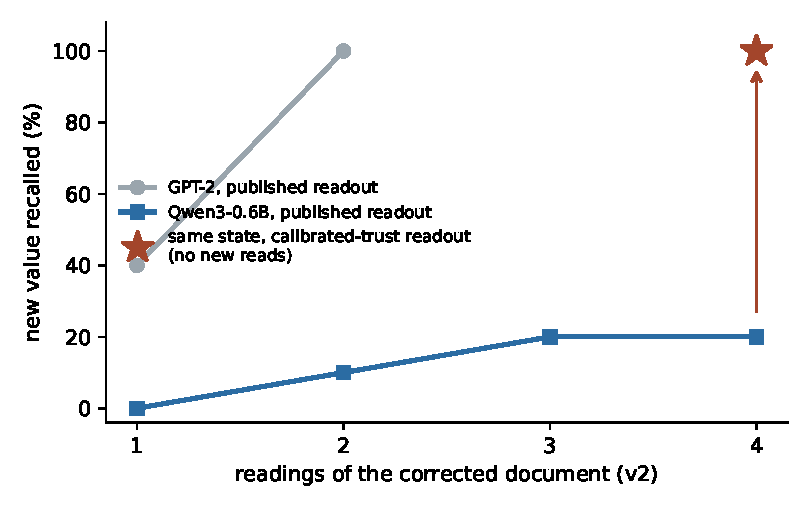
\includegraphics[width=0.62\linewidth]{figs/p6fig1_trust.pdf}
\caption{Conflict resolution: recall of the corrected value vs readings of the correcting document. GPT-2 flips in two readings; Qwen3 plateaus at 20\% under its published readout ($\lambda_G = 0.2$) --- and jumps to 100\% on the \emph{same state, with no new reads}, when probed under a high-trust readout ($\lambda_G = 0.85$). The storage had the answer; the readout spoke too softly.}
\label{fig:trust}
\end{figure}

Figure~\ref{fig:trust}: under Qwen3's published readout settings ($\beta{=}160$, $\lambda_G{=}0.2$, abstention $q_{75}$), recall of corrected values crawls --- 0\%, 10\%, 20\%, 20\% after one to four readings of the correcting document, with the confusion share at 80--100\% (the old value is at 0\% throughout: it died immediately, as on GPT-2). The natural reading is a storage failure. It is not. Probing the \emph{same state}, with \emph{zero further reads}, under the high-trust settings that read-only calibration selects for this family in \cite{drafter} ($\beta{=}40$, $\lambda_G{=}0.85$, $q_{50}$): corrected-value recall goes to \textbf{100\%}, confusion to 0\% --- and the two residual failures of stable-fact recall (93\%) disappear as well (100\%). The memory had resolved the conflict; the readout's interpolation weight was too small for its resolution to flip the argmax.

We offer this as the unifying mechanism for three observations that the series had reported separately: kNN-LM improves likelihood on every stream of \cite{sillage} yet never moves top-1 decisions (its tuned $\lambda$ is 0.05--0.1); the semantic tier of \cite{router} improves likelihood but not greedy recall at its tuned weights ($\lambda_S \le 0.1$); and calibrating the readout for a bigger sibling is what converts drafting confidence into accepted tokens in \cite{drafter}. One knob --- how much the mixture trusts the memory --- governs the conversion of nats into behavior, everywhere. Two honesty notes: the high-trust probe borrows settings selected by \cite{drafter}'s calibration procedure rather than re-deriving them on this stream (it is mechanistic evidence, not a recommended constant); and trust is not free in general --- which is why the next two subsections measure exactly what it does and does not cost.

\subsection{Two boundaries of different natures}\label{sec:boundaries}

Paraphrase recall is 0\% in every configuration tested: GPT-2, Qwen3 with its semantic tier active, and --- decisively --- Qwen3 under the same maximal-trust readout that unlocked conflict resolution. Trust does not touch it, because nothing is retrieved to trust: the never-seen template shares no $n$-gram with the stored one, and at its tuned weights the semantic tier redistributes likelihood without flipping argmaxes (the behavioral face of \cite{router}'s own honest finding). The two classic failure modes of this memory are therefore of different kinds --- \textbf{conflicts fail in the readout; paraphrase fails in the keys} --- and interventions aimed at one cannot repair the other. The suite separates them with two knobs: one probe template and one interpolation weight.

\subsection{Locality, decomposed to the mechanism}\label{sec:locality}

\begin{table}[t]
\centering\small
\caption{Locality on the natural-prose witness (Qwen3 state after the full conflict history; teacher-forced, nothing written). The drift is invariant to the memory's interpolation weight --- and vanishes with the adapter.}
\label{tab:locality}
\begin{tabular}{@{}lc@{}}
\toprule
configuration & witness PPL drift\\
\midrule
full system & $+$4.00\%\\
without the adapter & $+$0.11\%\\
without adapter and semantic tier & $\pm$\textbf{0.00\%}\\
adapter only (semantic off) & $+$3.88\%\\
\bottomrule
\end{tabular}
\end{table}

The $+$4.0\% witness drift on Qwen3 (Table~\ref{tab:suite}) decomposes cleanly (Table~\ref{tab:locality}): the Hebbian memory's contribution is \emph{exactly zero} --- its confidence never once clears the abstention threshold on unrelated prose, which an independent measurement confirms (witness perplexity is identical to the second decimal under $\lambda_G = 0.2$ and $0.85$: the gate never opens, so the weight never matters). Essentially the whole drift is the rank-16 adapter ($+$3.88\% alone): its delta-rule recalibration of the readout, which buys the broad in-domain gains of \cite{fw}, has an out-of-domain price that \cite{fw} did not measure. The memory is a scalpel; the adapter is diffuse. For deployments where locality is a requirement, the adapter --- not the memory --- is the component to gate.

\subsection{Who carries retention: working memory vs durable memory}\label{sec:whocarries}

\begin{figure}[t]
\centering
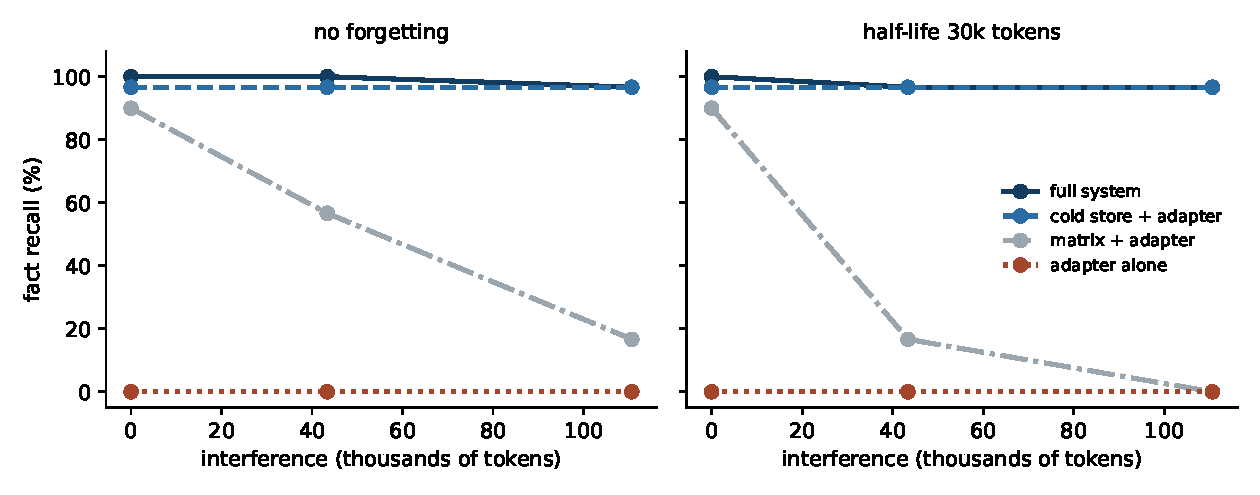
\includegraphics[width=\linewidth]{figs/p6fig3_retention.pdf}
\caption{Fact recall under interference, decomposed into four voices (GPT-2). The full system holds at 97\%; alone, the matrix erodes even without forgetting and collapses to zero under it; the cold store $+$ adapter holds 97\% throughout both arms; the adapter alone recalls nothing. The durable memory of this system is the consolidated exact store.}
\label{fig:whocarries}
\end{figure}

Figure~\ref{fig:whocarries} answers the question the retention numbers raise: recall survives 110k tokens of interference at 97\% --- but \emph{who} carries it? Four probes per checkpoint (full; cold store disabled; matrix silenced via $\lambda_G{=}0$; both off) across two arms:

\begin{itemize}[leftmargin=1.4em,itemsep=1pt]
\item \textbf{The matrix is working memory.} Without the cold store it starts at 90\% and erodes to 57\% ($+$43k) and 17\% ($+$110k) \emph{with no forgetting enabled}: fact amplitudes are fixed while superposition noise grows as $\sqrt{N}$ with interference writes --- the conditioning argument of \cite{sillage}, seen from its dark side. With a 30k-token half-life it reaches 0\%.
\item \textbf{The cold store is durable memory.} Cold $+$ adapter holds 97\% at every checkpoint of both arms. Consolidation-by-surprise \cite{hier} is not an optimization; behaviorally, it \emph{is} the long-term memory.
\item \textbf{Forgetting is therefore behaviorally free}: the full system's recall is identical with and without decay (97\%), because the tier that decays is not the tier that retains --- the hierarchy as retention insurance, quantified.
\item \textbf{The adapter memorizes nothing} (0\% at every point): facts live in the memory, style in the readout --- the division of labor of \cite{fw}, now tested at the level of individual facts.
\end{itemize}

\subsection{The two-occurrence rule}\label{sec:twoocc}

\begin{table}[t]
\centering\small
\caption{The admission threshold as a behavioral law (GPT-2). Groups of ten facts seen once, twice, three times in one graded dossier; interference as in \S\ref{sec:whocarries}. ``Cold coverage'': facts whose probe $n$-gram the cold store can answer (admission requires $\ge 2$ occurrences).}
\label{tab:twoocc}
\begin{tabular}{@{}lccc@{}}
\toprule
& seen $\times$1 & seen $\times$2 & seen $\times$3\\
\midrule
cold coverage & \textbf{0/10} & 10/10 & 10/10\\
recall at $+$0k & 100\% & 100\% & 100\%\\
recall at $+$43k & \textbf{0\%} & 90\% & 100\%\\
recall at $+$110k & \textbf{0\%} & 90\% & 100\%\\
final recall, cold disabled & 0\% & 20\% & 30\%\\
\bottomrule
\end{tabular}
\end{table}

Table~\ref{tab:twoocc} turns a design constant into a law. Facts seen once never clear the cold store's admission gate (\texttt{COLD\_MIN\_COUNT}$\,=2$): they live on the working memory alone, are recalled perfectly at first --- and are gone by $+$43k tokens. Facts seen twice are admitted, and are retained at 90\% through $+$110k (three sightings: 100\%; the third occurrence still consolidates). The cold-disabled row confirms the attribution: the survivors are carried by the consolidated store. \textbf{This system durably remembers what it has seen twice} --- and the practical corollary for users is equally plain: re-reading is consolidation.

\subsection{Context equivalence: what is the state worth in tokens?}\label{sec:equiv}

\begin{figure}[t]
\centering
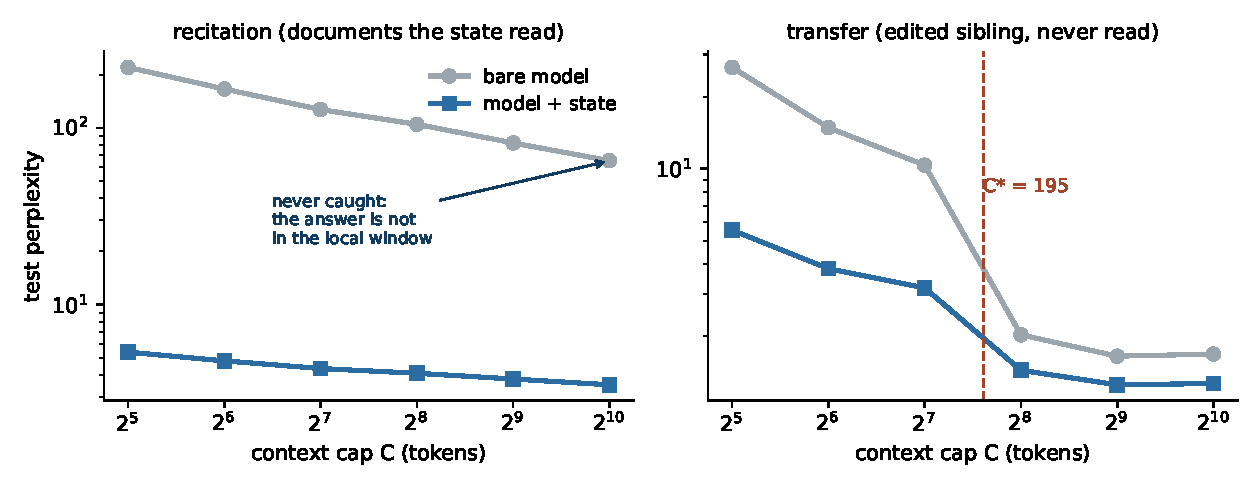
\includegraphics[width=\linewidth]{figs/p6fig2_equivalence.pdf}
\caption{The context-equivalence curves (GPT-2, papers state; teacher-forced, nothing written; scored positions identical across caps). Left --- \emph{recitation} (a tail segment of the documents the state read): the bare model never reaches memory$+$64-tokens even at $C{=}1024$. Right --- \emph{transfer} (an edited sibling document never read): the bare model needs $C^{*} = 195$ tokens to match memory$+$64, and the memory still helps at full context.}
\label{fig:equiv}
\end{figure}

Define $C^{*}$ as the context cap at which the \emph{bare} model's teacher-forced NLL matches the \emph{augmented} model's at a 64-token cap --- ``how many tokens of context is the state worth?''. Figure~\ref{fig:equiv} gives the two regimes. On \emph{recitation} --- re-accessing documents the state has read --- the question has no finite answer: memory$+$64 sits at perplexity 4.8 while the bare model is still at 65 with $C = 1024$ ($16\times$ more context, $13\times$ worse). The reason is structural, not quantitative: the predictive information lives elsewhere in the 22k-token corpus, outside any local window --- \textbf{local context cannot substitute for cross-document memory}. On \emph{transfer} --- an edited sibling never read --- $C^{*} = 195$: the bare model can catch up, at three times the token budget, by exploiting the document's own internal repetition; and even at $C = 1024$ the memory still improves perplexity by 25\% (1.27 vs 1.69). $C^{*}$ is segment-dependent by design --- that it \emph{discriminates} regimes is precisely its value as a metric.

\subsection{Adversarial interference: the gate prices the attack}\label{sec:adversarial}

\begin{table}[t]
\centering\small
\caption{Direct collision attack (GPT-2): ``The \{probed entity\} protocol requires \emph{further inspection}.'' written at the facts' own addresses, dosed against the facts' 3 occurrences. Arm B (same template, 60 \emph{other} entities, matched volume) is the selectivity control.}
\label{tab:adv}
\begin{tabular}{@{}lccc@{}}
\toprule
& true value & distractor & neither\\
\midrule
arm B: other entities ($\approx$dose 9) & \textbf{100\%} & --- & ---\\
collision dose 1 (vs 3) & 100\% & 0\% & 0\%\\
collision dose 3 (parity) & \textbf{93\%} & 3\% & 3\%\\
collision dose 9 ($3\times$ the mass) & 50\% & 50\% & 0\%\\
dose 9, cold store disabled & 33\% & \textbf{0\%} & 67\%\\
\bottomrule
\end{tabular}
\end{table}

Table~\ref{tab:adv}: selectivity holds at the edge (arm B: sixty sibling entities in identical sentences leave recall untouched --- the entity pieces are in the key, so the addresses differ). The direct collision --- the one theoretically valid attack, writing a competing successor at the exact value-predicting $n$-gram --- degrades recall far more slowly than raw bookkeeping predicts: at write parity the true value still wins 93/3, and the behavioral tipping point (50/50) needs \emph{three times} the fact's mass. Disabling the cold store at dose 9 is the decisive row: \textbf{the distractor drops to 0\%} --- the amplitude matrix never surrenders to it (it blurs the address into confusion instead), and the entire attack was carried by the cold tier's counts.

Why does the matrix resist? Our first measurement flattered the system so much (a 13:1 score ratio for the true value where amplitude arithmetic predicts 0.58:1 \emph{against} it) that we treated it as an artifact and instrumented the write path itself. The trace exonerated the amplitude rule --- final amplitudes match $\sqrt{\text{effective mass}}$ to the second decimal --- and exposed the real mechanism: \textbf{the surprise gate deduplicates the attack}. Collision sentences repeated within the frozen model's context window become predictable by in-context copying, and their write gates collapse from 5.0 to 0.05--0.09 by the third repetition; nine attack writes purchased $\approx$15 units of mass instead of 45. The effect has a measurable geography: the first entity in each collision block (attacked ``fresh'' after filler) ends with a distractor score of 0.744, the third 0.10, the last five average 0.026. \emph{In-window redundancy is free for the defender}: to inject mass, an attacker must spread collisions across windows, multiplying their token budget.

The vulnerable channel is now exactly identified: the cold store's successor counts are the one gate-blind quantity in the system --- every occurrence counts as 1 regardless of surprise --- and a naive repair (square-rooting the counts) measurably fails (50/50 unchanged: $\sqrt{9}{:}\sqrt{3}$ still outvotes at a fixed mixing weight). The principled fix follows the series' own design language: store \emph{surprise mass per successor} and serve the cold distribution from it --- the free signal's fourth job \cite{hier}. It has since shipped as the tool's opt-in \texttt{--cold-mass} mode (release 1.2.0; admission is untouched, so the two-occurrence rule and every number in this paper are unchanged, and counts remain the default). The honest statement stands: the memory's strength (durable retention, \S\ref{sec:whocarries}) and its attack surface are the same component --- the upgrade now exists, and re-measuring the collision table under it is the natural next probe.

\section{The laws at capacity}\label{sec:capacity}

Version 2 asks the question every reader of \S\ref{sec:trust} should ask: is the conversion failure just the smallness of the reader? The test holds storage constant and grows capacity: one state, written once by Qwen3-0.6B (dossier v1 then the correcting v2 twice; 8{,}922 tokens, 735 cold grams), is served by Qwen3-0.6B, 1.7B and 4B --- a $6.7\times$ parameter range with a shared tokenizer \cite{drafter}. The serving stack is reduced identically at every size to the $n$-gram and cold tiers: the semantic tier and the adapter are functions of the \emph{reading} model's hidden geometry (the same reason \cite{drafter} disables the adapter under cross-model serving), so keeping them would compare different systems. Predictions were registered before the run, including the falsification threshold: published-trust conflict resolution $\geq 50\%$ at 4B would have weakened the first law. The run is a single self-contained GPU kernel (fp16 forwards for 4B; float32 otherwise), released with the repository.

\begin{table}[t]
\centering\small
\caption{The capacity test: one 0.6B-written state, three family members serving it under an identical reduced stack. Conflict resolution (the updated value, 10 changed facts) and stable recall (the 20 untouched facts), at the state's published readout and at the family-calibrated readout of \cite{drafter}.}
\label{tab:capacity}
\begin{tabular}{@{}llccc@{}}
\toprule
readout & metric & 0.6B & 1.7B & 4B\\
\midrule
published $(\beta{=}160,\lambda{=}0.2,q75)$ & new value & 10\% & 10\% & 10\%\\
 & stable recall & 90\% & 80\% & 90\%\\
calibrated $(\beta{=}40,\lambda{=}0.85,q50)$ & new value & \textbf{100\%} & \textbf{100\%} & \textbf{100\%}\\
 & stable recall & 100\% & 95\% & 95\%\\
\bottomrule
\end{tabular}
\end{table}

Table~\ref{tab:capacity} is two flat lines. At the published readout, conflict resolution is 10\% at every size --- the falsification threshold was never approached --- and at the calibrated readout it is 100\% at every size. \textbf{Capacity does not buy conversion; trust does, and the effect of trust is capacity-invariant.} Stable recall is flat-to-noisy (90/80/90 published), not rising: a $6.7\times$ larger language prior neither rescues the timid readout nor disturbs the confident one.

The native arm sharpens the law further. Qwen3-4B reading its own dossier (full stack minus the semantic tier, which lacks a whitening for this geometry) reproduces the 0.6B behavioral profile almost exactly: empty-memory controls 0\%, free recall 93.3\% (identical to 0.6B's), paraphrase 0\% under every setting, witness drift $+0.47\%$, and a conflict plateau at 0\% after two corrective readings. The interesting detail is \emph{where} its trust dial lives: the readout governing the 4B reads already carries the family's $\beta{=}40,\lambda{=}0.85$ --- only the abstention threshold differs (q75 vs q50) --- and lowering that single notch takes conflict resolution from 0\% to 100\% (old value 0\%), with the 20 stable facts at 100\%. At this scale the entire trust problem of \S\ref{sec:trust} compresses into one component: \emph{the abstention threshold is the trust dial}.

Two honest negatives from the pre-registration: stable published recall at 1.7B (80\%) fell below our declared $\geq 85\%$ bound, and the predicted weak growth of served recall with capacity did not appear (the axis is flat). Neither touches the law; both are recorded in the released log with the predictions they missed.

\section{Discussion}

\textbf{An anatomy, not a scoreboard.} Six laws now describe this system's behavior: recall converts through trust; paraphrase fails in the keys; the matrix works, the cold store remembers, the adapter styles; twice-seen is durably kept; context substitutes for memory only within a document; and surprise prices attacks as it prices writes. Version 2 adds the capacity rider: none of this moves when the reader grows $6.7\times$ (\S\ref{sec:capacity}). None of these is visible in a perplexity table, several cut \emph{against} the system (paraphrase; the adapter's locality price; the cold tier's attack surface), and each is attributed to a mechanism that a designer can act on. This is what we believe behavioral evaluation is for --- not a leaderboard number, but laws with handles.

\textbf{Design consequences.} Three follow directly. The trust knob should track state maturity --- the read-only calibration of \cite{drafter} already ships in the tool, and \S\ref{sec:trust} shows what it unlocks behaviorally. Locality-critical deployments should gate the adapter, not the memory (\S\ref{sec:locality}). And the cold tier should mass-weight its successors (\S\ref{sec:adversarial}) --- one change serving robustness and, likely, conflict resolution at once; it shipped in release 1.2.0 as \texttt{--cold-mass}, counts remaining the default.

\textbf{A methodological note.} Two findings in this paper began as measurements too favorable to trust: a 13:1 resistance ratio, and a retention curve that barely moved. Both survived only after being instrumented to the mechanism (write-level traces; four-voice decompositions), and one dissolved into a better finding than the artifact it replaced. We would generalize the habit: \emph{when a behavioral result flatters the system, instrument the writes before citing it.}

\section{Limitations}

Synthetic facts in templated filler (ecological validity is bounded; the paraphrase 0\% in particular is measured on one unseen template family); two small models (124M, 0.6B) and one behavioral run per configuration under fixed seeds (deterministic replication, but no seed variance); greedy probes with an 8-token window; interference is same-register filler (a soft regime --- the adversarial section is the hard one); the high-trust probe borrows \cite{drafter}'s calibrated settings rather than re-deriving them per protocol; $C^{*}$ depends on the scored segment's self-predictability (by design, but it forbids single-number claims); the cold-tier fix has shipped (1.2.0, opt-in) but the collision table is not yet re-measured under it; the capacity test serves a reduced stack ($n$-gram + cold) with one run per configuration, and its native 4B arm has no semantic tier by construction; and the external benchmark stage --- LongMemEval \cite{longmemeval} --- is now measured in the seventh preprint of this series \cite{bench}, for which this paper supplies the mechanism-level ground truth.

\section{Conclusion}

A memory can hold the right answer and still not say it. Across a gradient-free memory system we measured where storage and behavior part ways --- the readout's trust, the keys' surface, the admission gate, the local window, the price of surprise --- and each divergence resolved into a law with a mechanism and a handle. The oldest distinction in the memory literature, between storage and retrieval, turns out to be an engineering variable in frozen-model memories: \emph{stored is not recalled}, and the difference is measurable, attributable, and adjustable.

\appendix

\section{Reproduction}

\begingroup\emergencystretch=2.5em\hbadness=1900
Scripts (released alongside the repository): \texttt{behavioral.py} (the six-probe suite and the no-write witness scorer), \texttt{retention.py}, \texttt{cold\_retention.py} (four-voice decomposition), \texttt{two\_occurrences.py}, \texttt{equivalence.py} (the $C^{*}$ scorer; transfer variant included), \texttt{adversarial.py} and its defense/decomposition probes, plus the \texttt{amp\_write} instrumentation used in \S\ref{sec:adversarial}. Committed results: thirteen JSON files under \texttt{results/} with the \texttt{behav\_} prefix, one per experiment, including per-fact detail rows. Settings: 30 facts, values probed by 8-token greedy completion of the canonical prefix; dossier repeats each fact $\times$3 unless graded; interference steps of $\approx$21k tokens; witness scored teacher-forced with windows 1024/512; conflict document v2 changes 10 values; collision distractor ``further inspection''; all list seeds fixed in code; figures regenerate via \texttt{figures/make\_figures\_p6.py}. Predictions for each experiment were written in the released log before running it. Version 2 adds the capacity kernel \texttt{behav/kaggle\_4b/} (self-contained: the invented-fact dossier is rebuilt on device, no state or document ships with it; fp16 forwards for 4B) and its committed result \texttt{results/behav\_4b.json}, predictions --- including the declared falsification threshold --- registered in the same log before the run.\par\endgroup

\begin{thebibliography}{17}\small

\bibitem{sillage} A.~Sghairi. Sillage: Surprise-gated amplitude memory for frozen language models. Preprint, 2026. \href{https://doi.org/10.5281/zenodo.22079016}{doi:10.5281/zenodo.22079016}.

\bibitem{router} A.~Sghairi. Route the scores, not the keys: Gradient-free semantic memory for frozen language models. Preprint, 2026. \href{https://doi.org/10.5281/zenodo.22079444}{doi:10.5281/zenodo.22079444}.

\bibitem{hier} A.~Sghairi. One signal, three tiers: A routed memory hierarchy with surprise-gated consolidation. Preprint, 2026. \href{https://doi.org/10.5281/zenodo.22079471}{doi:10.5281/zenodo.22079471}.

\bibitem{fw} A.~Sghairi. Memory remembers, fast weights adapt: Two gradient-free ways to learn at test time, and why they add up. Preprint, 2026. \href{https://doi.org/10.5281/zenodo.22079481}{doi:10.5281/zenodo.22079481}.

\bibitem{drafter} A.~Sghairi. The memory pays for itself: Cross-model recall and exact speculative acceleration from one fixed-size Hebbian state. Preprint, 2026. \href{https://doi.org/10.5281/zenodo.22109220}{doi:10.5281/zenodo.22109220}.

\bibitem{bench} A.~Sghairi. Found is not formulated: A gradient-free memory meets LongMemEval. Preprint, 2026. \href{https://doi.org/10.5281/zenodo.ZZDOI7}{doi:10.5281/zenodo.ZZDOI7}.

\bibitem{beyondppl} X.~Song, Z.~Chen, L.~Kong, S.~Xie, X.~Dong, G.~Chen, K.~Zhang. Beyond perplexity: A behavioral evaluation framework for deployment-memory claims in LLM test-time training. arXiv:2607.00368, 2026.

\bibitem{khandelwal2020} U.~Khandelwal, O.~Levy, D.~Jurafsky, L.~Zettlemoyer, M.~Lewis. Generalization through memorization: Nearest neighbor language models. \emph{ICLR}, 2020.

\bibitem{rome} K.~Meng, D.~Bau, A.~Andonian, Y.~Belinkov. Locating and editing factual associations in GPT. \emph{NeurIPS}, 2022.

\bibitem{memit} K.~Meng, A.~S.~Sharma, A.~Andonian, Y.~Belinkov, D.~Bau. Mass-editing memory in a transformer. \emph{ICLR}, 2023.

\bibitem{longmemeval} D.~Wu, H.~Wang, W.~Yu, Y.~Zhang, K.-W.~Chang, D.~Yu. LongMemEval: Benchmarking chat assistants on long-term interactive memory. \emph{ICLR}, 2025.

\bibitem{mcclelland} J.~L.~McClelland, B.~L.~McNaughton, R.~C.~O'Reilly. Why there are complementary learning systems in the hippocampus and neocortex. \emph{Psychological Review}, 102(3):419--457, 1995.

\bibitem{kumaran} D.~Kumaran, D.~Hassabis, J.~L.~McClelland. What learning systems do intelligent agents need? \emph{Neuron}, 89(1):1134--1152, 2016.

\bibitem{titans} A.~Behrouz, P.~Zhong, V.~Mirrokni. Titans: Learning to memorize at test time. arXiv:2501.00663, 2025.

\bibitem{ttt} Y.~Sun, X.~Li, K.~Dalal, J.~Xu, A.~Vikram, G.~Zhang, Y.~Dubois, X.~Chen, X.~Wang, S.~Koyejo, T.~Hashimoto, C.~Guestrin. Learning to (learn at test time): RNNs with expressive hidden states. arXiv:2407.04620, 2024.

\bibitem{gpt2} A.~Radford, J.~Wu, R.~Child, D.~Luan, D.~Amodei, I.~Sutskever. Language models are unsupervised multitask learners. OpenAI Technical Report, 2019.

\bibitem{qwen3} A.~Yang et al. Qwen3 technical report. arXiv:2505.09388, 2025.

\end{thebibliography}

\end{document}
